\section{Accounting Properties and Metric Definitions}
\label{app:properties}
\paragraph{Event identity and retries.}
Each physical request and execution event has an identifier. For a set of unique new events $N$, the incremental work is $\Delta\W=\sum_{e\in N}\mathbf{w}(e)$. A replayed log entry contributes once; a physically repeated operation receives a new identity and contributes again. Imported prefix events carry their prior work separately and have zero new-resource delta. Thus concatenating a prefix and continuation gives $\W_{0\rightarrow u}=\W_0+\Delta\W_u$ without double counting.

\paragraph{Units.}
Let $a_j>0$ convert coordinate $j$ to another unit. Multiplying both workflows' coordinate by $a_j$ preserves every inequality in Equation~\ref{eq:dominance}, hence preserves dominance and trade-offs. For a positive denominator it also preserves $1-a_jW_j(\ell)/(a_jW_j(h))=S_W$. These properties explain why no cross-resource weighting is needed. They do not turn different work coordinates into interchangeable quantities.

\paragraph{Timing.}
For interval sets $I_M,I_W$, inclusion--exclusion gives $|I_M\cup I_W|=U_M+U_W-O$. Subtracting this active union from the elapsed runtime yields the residual. Concurrent worker durations are never summed to represent wall time. The native replay statistic is $|I_W|$, measured again for each replay; the online statistic is elapsed runtime through completion. Search, scoring, and the verifier's evidence re-execution are separate evaluator costs.

\paragraph{SQL work proxy.}
The implementation calls SQLite's progress handler every 1,000 virtual-machine instructions. The legacy field is named \nolinkurl{sqlite_vm_steps_lower_bound}; the paper reports callbacks or callbacks multiplied by 1,000 as a progress-work proxy. Short queries can produce zero callbacks, and SQLite's callback behavior can depend on preparation and version. This field is not an exact instruction counter or a guaranteed universal lower bound. A14's 19.5 ratio is 39/2 callbacks, not an asserted 19.5-fold runtime ratio.

The declared primary coordinates are graph paper records read, native regression cases executed, SQLite progress-work units, metric values read, and business records read, respectively. All other recorded native coordinates remain in the dominance test. Zero primary-work denominators are excluded from ratio calculations and remain visible as absolute measurements in the component tables.

\begin{table*}[t]
\centering\small
\begin{tabular}{p{.19\textwidth}p{.36\textwidth}p{.36\textwidth}}
\toprule
Measurement & Definition & Interpretation\\
\midrule
Submission & Evaluated final submissions / planned stages & Interface completion; unsuccessful answers remain submitted.\\
$Q_1$, $Q_2$, $\G$ & Output validity; support/state validity; their conjunction & Separates a plausible result from an executable, supported result.\\
Native work & Event-summed vector, with domain units & Distinguishes broad scans, repeated checks, shared work, writes, and transformations.\\
Work relation & Equal, dominant, or incomparable vector & Identifies resource improvement and explicit trade-offs.\\
$S_W$, $S_T$, $D$ & Work saving, time saving, and $S_W-S_T$ & Measures the extent to which a native saving is realized in a specified timing domain.\\
$A_{\rm rel}$, $A_{\rm irr}$ & Valid continuations / valid initial executions & Measures repair and preservation from each model's completed states.\\
Incremental resources & New work, requests, elapsed time, and receipts & Reveals the cost of adaptation and reuse.\\
Prefix audit & Recheck old answer and old evidence under the new task & Separates changed output, fresh evidence, and reusable state.\\
\bottomrule
\end{tabular}
\caption{Metric dictionary. The quality aggregate averages one binary gate; it does not combine quality, cost, time, and adaptation into a weighted score.}
\end{table*}

\section{Detailed Source Construction}
\label{app:sources}
\paragraph{Graph sources.}
The STaRK source revision is \nolinkurl{88269e23e90587f99476c5dd74e235a0877e69be}. The original slice contains 16,550 nodes and 149,765 edges. The Stanford, MIT, and Tokyo slices contain 16,058/142,401, 14,376/126,927, and 13,167/120,386 nodes/edges. Expansion sampling selects authors from declared institutions, retains their authored publications and outgoing references, and records the seed. Focal authors do not overlap the original selection; reference nodes do. Parent allocation is 8/4/4/4 across these four clusters. Task membership and source hashes are provided in the catalog.

\paragraph{Code sources.}
Requests is pinned at commit \nolinkurl{b25c87d7cb8d6a18a37fa12442b5f883f9e41741}; ItsDangerous at \nolinkurl{096c8d42545d3b68ea21a4f890fb2b2d8979c0bd}. packaging and python-dotenv use published 25.0 and 1.1.1 source archives with SHA-256 receipts. Parent allocation is 4/4/6/6. We keep original, seeded, and repaired snapshots separately. Public inputs and expected case behavior are distinct from observed current behavior. Checks bind package, check ID, case ID, and current revision. A valid review must identify exactly the failing scoped cases. Code mutations are experimental changes, not claims of defects in the cited releases.

\paragraph{Relational sources.}
The first eight analytics parents use BIRD mini-dev debit and financial databases, four each. Six Chinook and six Northwind parents extend the suite. Consumption tasks aggregate a declared year and requested customers. Loan tasks aggregate requested regions and statuses. Purchase tasks count distinct invoices/orders, sum line quantities, and sum price times quantity; Northwind applies line discounts. Requested customer IDs retain their source type. Updates alter the object set or a controlled source value. Native summary functions and equivalent read-only SQL can both satisfy the contract.

\paragraph{Telemetry sources.}
RCAEval expansion files are pinned at Hugging Face revision \nolinkurl{afeacb11bcc94dadfd1c8f483ee4377b2b8b614e}. The original checkout cluster supplies eight parents; currency CPU, product-catalog delay, and Train Ticket order CPU incidents supply four each. Each source preserves metrics, logs, traces, and an injection-time file. Public split timestamps and filters determine expected quantities. Relevant cards shift the split while leaving raw source records unchanged. The transformation creates observable diagnostic reports from RCAEval, rather than reusing its original root-cause ranking score.

\paragraph{Application sources.}
The exports are identified by AppWorld tasks \texttt{b0a8eae\_1}, \texttt{22cc237\_1}, \texttt{3fcc458\_1}, and \texttt{90adc3f\_1}, with 4/4/6/6 parents. The latter two exports contain six/four playlists, 32/43 payment requests, and 106 user records each. The adapter implements local transitions over these records. Playback admits any owned playlist meeting the stated duration. Downloads use set membership and preserve prior downloads. Payment reconciliation computes $\max(0,\mathrm{share}-\mathrm{paid})$ and replaces a request by member identity. Each transition is recorded as native work. The evaluator checks actual state instead of trusting the completion string.

\paragraph{Difficulty and changes.}
All five scenarios have five easy and fifteen medium parents. Easy tasks reduce output burden and the number of requested objects. Medium tasks increase composition and evidence scope while preserving feasible native helpers. Neither tier removes the opportunities to batch, overscan, reuse, or update. Irrelevant cards preserve the target contract; related cards explicitly announce their change. The medium tier supplies the primary work--time analysis, and easy results are retained in the released tables.

\section{Model and Execution Configuration}
\label{app:models}
All models are accessed through OpenRouter with recorded provider routes. Six are grouped as open-weight model families and four as closed APIs. This is endpoint-family metadata, not a comparison of local open-weight deployment against hosted inference. In particular, Qwen3.8 Flash denotes the production API route used in the logs. The raw route, provider, quantization metadata where available, and request parameters accompany each collection campaign.

The final extension uses Grok 4.3, MiniMax M3, Gemini 3.7 Flash, GPT-6 Luna, and GLM-5.3 Flash. GLM replaces Mistral Small 4 before any formal Mistral stage because of sustained provider rate limiting. Development checks freeze JSON-object output and reasoning settings before main collection. GLM, Gemini 3.7, and Luna use low reasoning; Grok and MiniMax use disabled reasoning. Earlier models retain their recorded compatible settings. Provider-default sampling is used for the two generation repeats. Four fixed native worker slots and decision limits of 12/8 are shared across the main tiered suite.

Local request admission changes are recorded as campaign segments. Online pair construction requires the same acquisition group and segment; GLM's delayed collection is a separate group. Early R6/R7 segment labels are reconstructed from their fixed collectors, with provenance recorded. Native replays run all ten models together after collection, with saved responses, one/four slots, and three repeats. The final isolated replay campaign uses Python 3.13.4 and SQLite 3.49.1. Plot and analysis dependencies are recorded separately.

\paragraph{Instrument repairs and audit.}
The final tiered contract checks pass 784 checks; an additional expansion suite passes 19 targeted checks, including equivalent SQL and incorrect entity/test binding. The evidence-equivalence suite passes 11 cases. A non-object answer guard converts malformed answer values to an empty rejected object; 20 malformed examples fail and the normal scoring branch is preserved. Frozen evidence-equivalence auditing accepts two MiniMax stages that the original evidence matcher rejected. It changes neither responses nor executed traces. Four transport-error placeholders are excluded from JSON-syntax counts and remain in the physical-request ledger.

The final five-model extension contains 3,000 logical stages and 3,008 physical stage attempts. Of the logical stages, 2,994 have an evaluated submission and six do not. Four physical requests retain unknown-charge reservations. Transport accounting, model-answer correctness, and submission are separate records. Historical raw attempts are retained with their replacement mapping. All final 6,000 logical stages have a final record.

\section{Additional Results and Denominators}
\begin{table*}[t]
\centering\small\setlength{\tabcolsep}{5pt}
\begin{tabular}{lrrrrrr}
\toprule
Model & Submitted & $Q_1$ & $\G$ & Initial $\G$ & Related $\G$ & Irrelevant $\G$ \\
\midrule
DeepSeek V4 Pro 0813 & 600/600 & 295/600 & 269/600 & 117/200 & 9/117 & 117/117 \\
Kimi K2.6 & 596/600 & 397/600 & 374/600 & 153/200 & 52/153 & 152/153 \\
Qwen3.8 Flash & 575/600 & 410/600 & 402/600 & 159/200 & 72/159 & 152/159 \\
Gemma 4 31B & 571/600 & 458/600 & 406/600 & 161/200 & 81/161 & 161/161 \\
GLM-5.3 Flash & 600/600 & 550/600 & 526/600 & 184/200 & 150/184 & 182/184 \\
MiniMax M3 & 600/600 & 97/600 & 52/600 & 19/200 & 0/19 & 19/19 \\
Gemini 3.8 Flash & 599/600 & 531/600 & 530/600 & 196/200 & 135/196 & 196/196 \\
Gemini 3.7 Flash & 600/600 & 537/600 & 534/600 & 197/200 & 140/197 & 197/197 \\
Grok 4.3 & 594/600 & 270/600 & 221/600 & 97/200 & 3/97 & 96/97 \\
GPT-6 Luna & 600/600 & 563/600 & 559/600 & 196/200 & 165/196 & 196/196 \\
\bottomrule\end{tabular}
\caption{Exact denominators. Submitted denotes an evaluated final submission. The final two columns require a valid initial stage. They are not the unconditional counts for the corresponding 200 update stages.}
\label{tab:counts}\end{table*}
\begin{figure*}[t]
\centering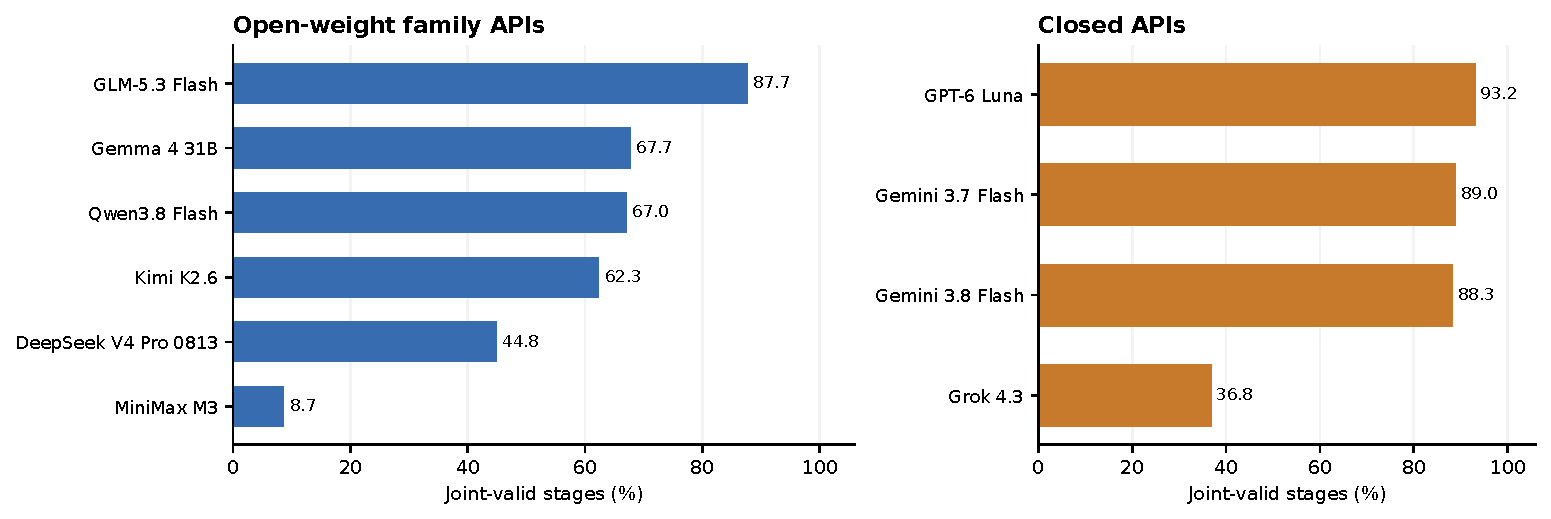
\includegraphics[width=.96\textwidth]{figure_5_validity.pdf}
\caption{Descriptive quality ranking within endpoint-family groups. Scores are valid-stage percentages over 600 stages. Work, time, and adaptation are reported separately and are not included in these bars.}
\end{figure*}

Across the initial, relevant, and irrelevant conditions, unconditional valid counts are 1,479, 862, and 1,532 out of 2,000 each. The conditional related and irrelevant counts are 807 and 1,468 out of 1,479. The difference arises because unconditional update outcomes also include continuations from initially invalid states. Exact per-model counts appear in Table~\ref{tab:counts}.

For one-worker native replay on medium tasks, 121/467 pairs show positive attenuation, 14/467 show nonpositive time savings, and 332/467 show at least proportional savings. The equal-parent mean gap is $-7.9$ points (95\% interval $[-15.6,1.0]$). At four workers the corresponding counts are 108, 27, and 332, with a mean gap of $-6.0$ points. These are different executions of fixed saved decisions. They diagnose timing layers without changing the generated workflow.

The same-pair comparison between four-worker native and online savings gives 41.3 points (24.4--61.1) before removing local admission and 24.2 points (13.9--34.5) afterward. Each statistic averages within a parent before averaging across the 37 eligible parents. Pair counts reflect available matched executions; they are not independent task counts.

Source-aware adaptation estimates average eligible repeats within parents, then use cluster-within-scenario and parent resampling. For Luna, the equal-parent relevant-update estimate is 83.3\% (76.7--89.7); for GLM it is 81.1\% (74.0--87.7). These differ slightly from the pooled conditional rates because a parent with one valid initial repeat receives the same parent weight as a parent with two. The release also provides every pairwise common-support adaptation table. Only eight parent--repeat cells have valid initial outcomes for all ten models, making that common intersection a small descriptive slice.

\section{Related-Work Coverage Evidence}
\label{app:coverage}
\begin{table*}[t]
\centering\small
\setlength{\tabcolsep}{3pt}
\begin{tabular}{lccccc}
\toprule
Evaluation & Executed outcome & Native work vector & Work--time pairing & Relevant updates & Valid-prefix cost\\
\midrule
WorFBench & $\circ$ & -- & -- & -- & --\\
FlowBench / FlowMind & $\checkmark$ & -- & -- & -- & --\\
AgentBoard & $\checkmark$ & -- & -- & -- & --\\
AppWorld & $\checkmark$ & -- & -- & -- & --\\
ClawArena-Team & $\checkmark$ & -- & -- & $\checkmark$ & --\\
OrchBench & $\circ$ & $\circ$ & $\circ$ & -- & --\\
\textbf{WELD} & $\checkmark$ & $\checkmark$ & $\checkmark$ & $\checkmark$ & $\checkmark$\\
\bottomrule
\end{tabular}
\caption{Reported coverage of the operational measurements used here. $\checkmark$: direct coverage; $\circ$: related coverage with a different measurement domain; --: no separately reported protocol of this definition in the inspected version. Native work vector retains heterogeneous execution units. Work--time pairing jointly measures native work and observed time for matched valid workflows. Valid-prefix cost measures new work from a validated completed checkpoint. WorFBench includes downstream execution; OrchBench reports simulated quality, makespan, and tokens. Appendix~\ref{app:coverage} gives the source mapping.}
\label{tab:coverage}
\end{table*}

Table~\ref{tab:coverage} maps reported protocols to the definitions in this paper. WorFBench v3 uses structural matching and includes downstream execution and timing experiments. FlowMind v1 evaluates task execution and reconstructed workflows, with token and tool-use analysis. AgentBoard reports progress and analytical evaluation, while AppWorld verifies application state. ClawArena-Team v2 reports execution-based task scoring, staged updates, permission/modality metrics, and usage analysis. OrchBench v1 evaluates quality, makespan, and token cost with a deterministic simulator. A related result is marked partial when its measurement domain differs from native execution. The table's final column specifically requires incremental cost from a validated completed prefix and a relevant/irrelevant contrast. This mapping concerns the reported measurements, not the theoretical capacity of their environments.

\section{Reproducibility Files}
The companion tables contain all 6,000 stages, all 5,006 initial pairs, component-level work, timing eligibility, prefix audits, adaptation pools, and source-aware sensitivity analyses. Figure scripts use these tables directly. Plans, revisions, observations, physical attempts, and frozen sources are indexed in the research archive. Task cards and evaluator source remain available independently of the run directories. All manuscript counts use the final audit.
